%%%%%%%%%%%%%%%%%%%%%%%%%%%%%%%%%%%%%%%%%%%%%%%%%%%%%%%%%%%%%%%%%%%%%%%%%%%%%%%%%%%%%%%%%%%%%%%%
%
% CSCI 1430 Written Question Template
%
% This is a LaTeX document. LaTeX is a markup language for producing documents.
% Your task is to answer the questions by filling out this document, then to
% compile this into a PDF document.
%
% TO COMPILE:
% > pdflatex thisfile.tex

% If you do not have LaTeX, your options are:
% - VSCode extension: https://marketplace.visualstudio.com/items?itemName=James-Yu.latex-workshop
% - Online Tool: https://www.overleaf.com/ - most LaTeX packages are pre-installed here (e.g., \usepackage{}).
% - Personal laptops (all common OS): http://www.latex-project.org/get/ 
%
% If you need help with LaTeX, please come to office hours.
% Or, there is plenty of help online:
% https://en.wikibooks.org/wiki/LaTeX
%
% Good luck!
% The CSCI 1430 staff
%
%%%%%%%%%%%%%%%%%%%%%%%%%%%%%%%%%%%%%%%%%%%%%%%%%%%%%%%%%%%%%%%%%%%%%%%%%%%%%%%%%%%%%%%%%%%%%%%%
%
% How to include two graphics on the same line:
% 
% \includegraphics[width=0.49\linewidth]{yourgraphic1.png}
% \includegraphics[width=0.49\linewidth]{yourgraphic2.png}
%
% How to include equations:
%
% \begin{equation}
% y = mx+c
% \end{equation}
% 
%%%%%%%%%%%%%%%%%%%%%%%%%%%%%%%%%%%%%%%%%%%%%%%%%%%%%%%%%%%%%%%%%%%%%%%%%%%%%%%%%%%%%%%%%%%%%%%%



\documentclass[10pt,twocolumn,letterpaper]{article}
\usepackage[T1]{fontenc}
\usepackage{cvpr}
\usepackage{times}
\usepackage{epsfig}
\usepackage{graphicx}
\usepackage{amsmath}
\usepackage{amssymb}
\usepackage{booktabs}
\usepackage{microtype}
\usepackage{subcaption}
% From https://ctan.org/pkg/matlab-prettifier
\usepackage[numbered,framed]{matlab-prettifier}

\frenchspacing

% Include other packages here, before hyperref.

% If you comment hyperref and then uncomment it, you should delete
% egpaper.aux before re-running latex.  (Or just hit 'q' on the first latex
% run, let it finish, and you should be clear).
\usepackage[pagebackref=true,breaklinks=true,letterpaper=true,colorlinks,bookmarks=false]{hyperref}

\cvprfinalcopy
\def\cvprPaperID{****}
\def\httilde{\mbox{\tt\raisebox{-.5ex}{\symbol{126}}}}
\ifcvprfinal\pagestyle{empty}\fi

\begin{document}

%%%%%%%%% TITLE
\title{CSCI 1430 Final Project Report\\Data Augmented AI Generated Detector}

% Make this document not anonymous
\author{Sujith Pakala, Sami Nourji, Everest Yang, Tanay Subramanian\\
    \emph{TA:} Winston Li \\
    Brown University\\
}

\maketitle
%\thispagestyle{empty}

%%%%%%%%% ABSTRACT
\begin{abstract}
    This paper explores an AI-generated image Detector to distinguish real images from AI-generated ones, addressing challenges posed by the rise of hyperrealistic content produced by generative AI. Using the CIFAKE dataset, we implement a CNN architecture with Fourier Transform features to evaluate their efficacy in identifying synthetic images. Our hypothesis is that incorporating frequency information via Fourier Transforms, in addition to spatial domain information, into a CNN can enhance the detection of AI-generated images by leveraging frequency inconsistencies. This was validated by our research, as our best-performing baseline CNN achieved a testing accuracy of 96.92\%, while our Fourier-based model reached an accuracy of 98.50\%. Our findings highlight the potential of leveraging Fourier Transforms for improved image classification, strengthening the growing field concerning digital authenticity.\end{abstract}

%%%%%%%%% BODY TEXT
\section{Introduction}

Misinformation and privacy are pressing concerns in today’s modern world. As chatbots and generative AI become more sophisticated, such technologies can create hyperrealistic fake images that are nearly impossible for an individual to discern. Misusing these innovative technologies has significant implications for politics, social trust, and even individual security. For example, AI-generated images have already been involved in election interference, celebrity impersonations, and malicious pranks, underscoring the importance of a model that reliably detects fake images.

Consequently, our project becomes essential for verifying digital content's authenticity as realistic synthetic images can now be generated in seconds. However, the central challenge to solving this problem is that AI-generated content can replicate minute details such as lighting, shadows, and texture with high precision, making conventional detection methods less effective. Furthermore, it is not feasible to manually label AI-generated content at scale, highlighting the importance of automated tools in detecting artificial images.

We became familiar with these types of images through both social media and exploratory generation with tools such as Stable Diffusion. After lengthy discussions on the subject, we noticed that AI-generated images display textures that appear smoother than ‘real images’. To test this theory, we decided to focus on AI-Generated image detectors, and introduce frequency domain information into the models through the Fourier Transform. This paper proposes a novel AI-Generated Image Detector to determine whether adding frequency domain information would enhance the model’s ability to discern real images from AI-generated ones. Studies have shown that AI-generated images have unique characteristics - such as specific frequency patterns, smooth texture, and artifacts - which distinguish them from real images. By applying Fourier Transforms, we can quantify these differences in the frequency domain where smoothness and periodic artifacts are more evident. This approach aims to enhance the model's robustness in detecting artificial images.

\section{Related Work}

The rapid growth of generative adversarial networks (GANs) has created opportunities and ethical concerns regarding the misuse of synthetic images. In recent academia, the CIFAKE dataset has become standard in distinguishing AI-generated images from real photographs.

This dataset was created by generating synthetic images using latent diffusion to mirror the ten classes of the CIFAR-10 dataset. The synthetic dataset was paired with real images. Using a CNN, the study achieved 92.98\% accuracy across 36 network topologies. Explainable AI techniques, using Gradient Class Activation Mapping, shows that the model focuses on small imperfections in the background instead of the main object \cite{1}\cite{2}. This dataset has been used for many AI-detection work, notably the 'Harnessing Machine Learning for Discerning AI-Generated Synthetic Images' paper by Wang et al. achieving a 97.74\% accuracy \cite{3}, as well as research by Lađević et al. using lightweight CNNs \cite{4}. The latter approach yielded similarly high results as the first paper, while only using four convolutional and two hidden layers to identify AI-generated images. This architecture was also tested on benchmark datasets and Sentinel-2 images, and outperforms four state-of-the-art methods with its lightweight architecture.

Our main contribution is the addition of Fourier Transform information to CNNs to enhance efficiency in image classification tasks. Based on their work, we integrated a Fourier Transform into our model to improve spatial-frequency feature extraction \cite{5}. By leveraging the Fourier Transform, it accelerates training times by up to 71\% with greater accuracy and reduced computational complexity. Given our limited hardware capabilities, we adopted their approach to balance accuracy and training time.


\section{Method}

\begin{figure}[htbp]
    \centering
    \begin{minipage}{0.4\textwidth} % Adjust width as needed
        \centering
        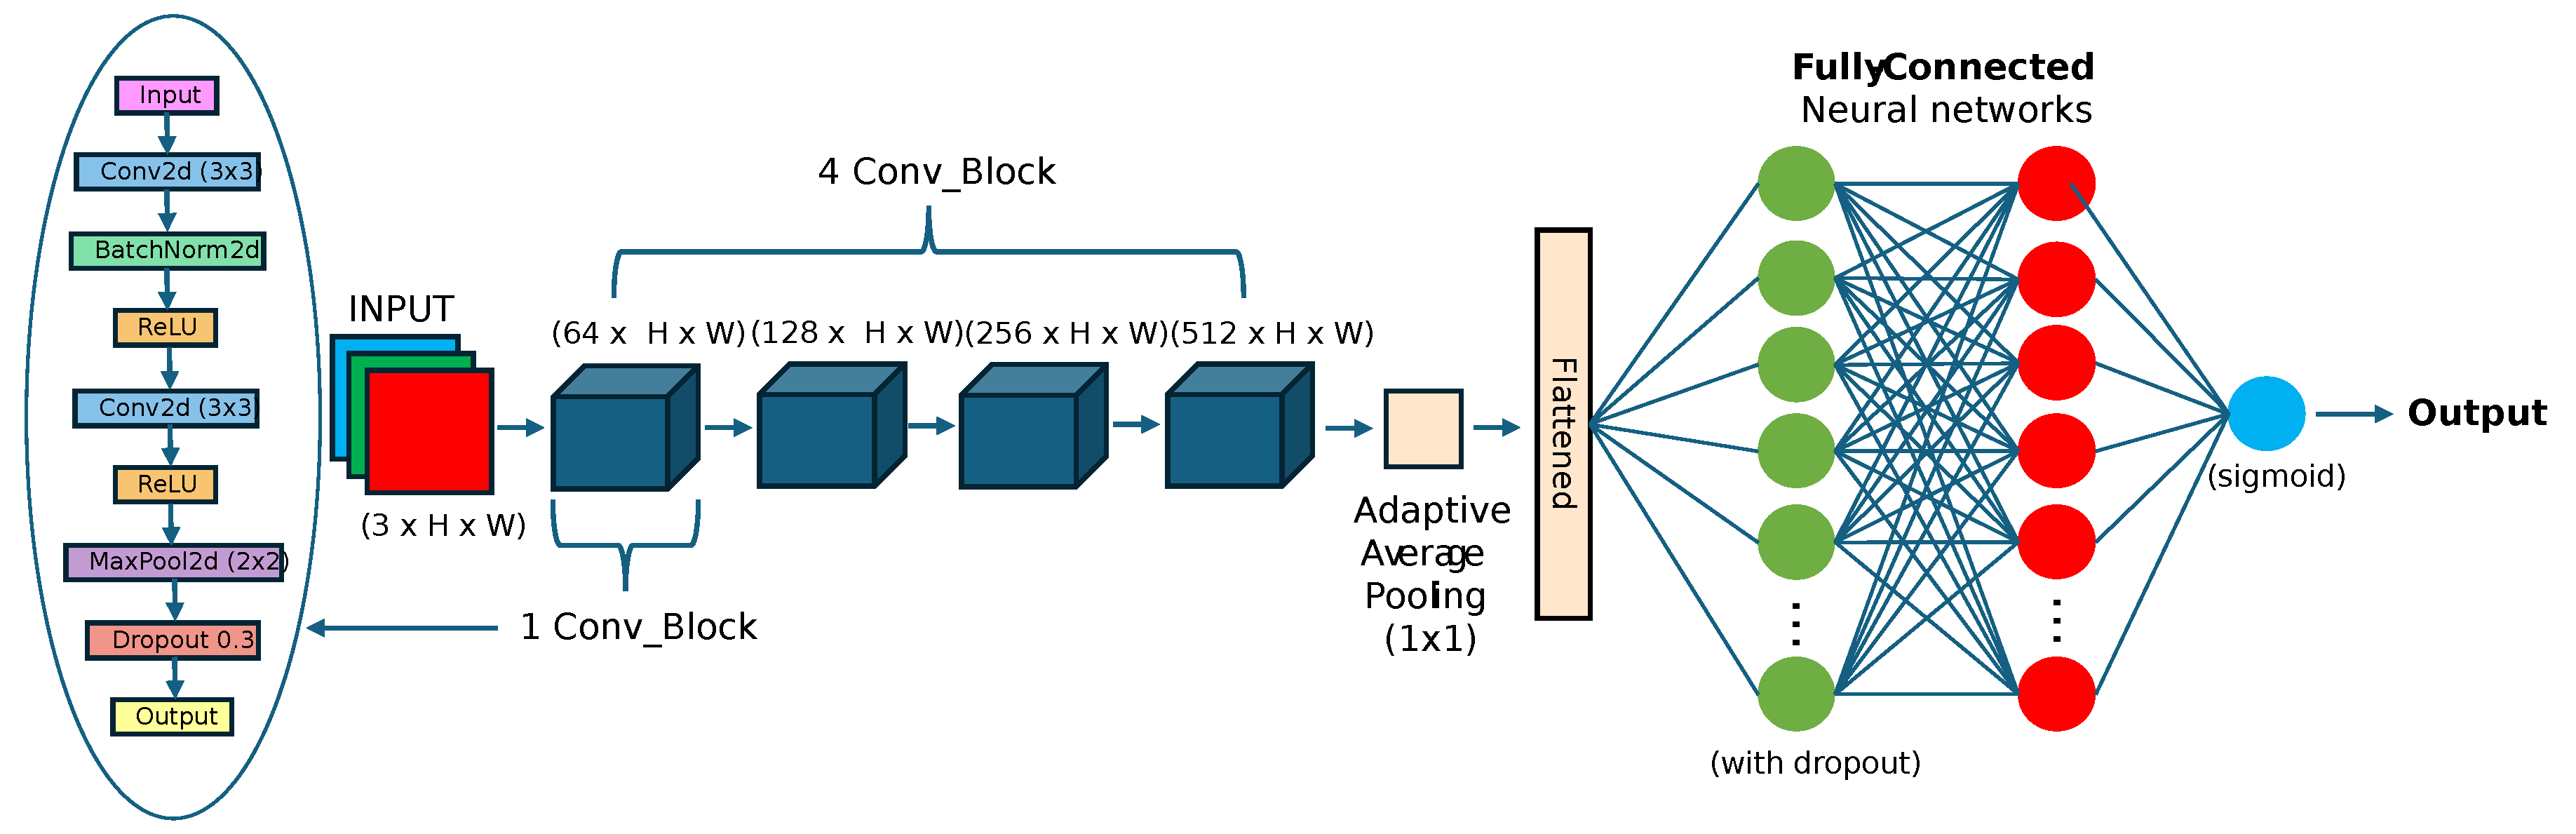
\includegraphics[width=\textwidth]{/Users/sami/Desktop/Brown/Classes/Fall 2024/CSCI 1430/CS1430_Projects/final-project-1430-CV/writeup/Images/ai-05-00076-g006.png}
        \caption{Original paper architecture}\label{fig:fig1}

        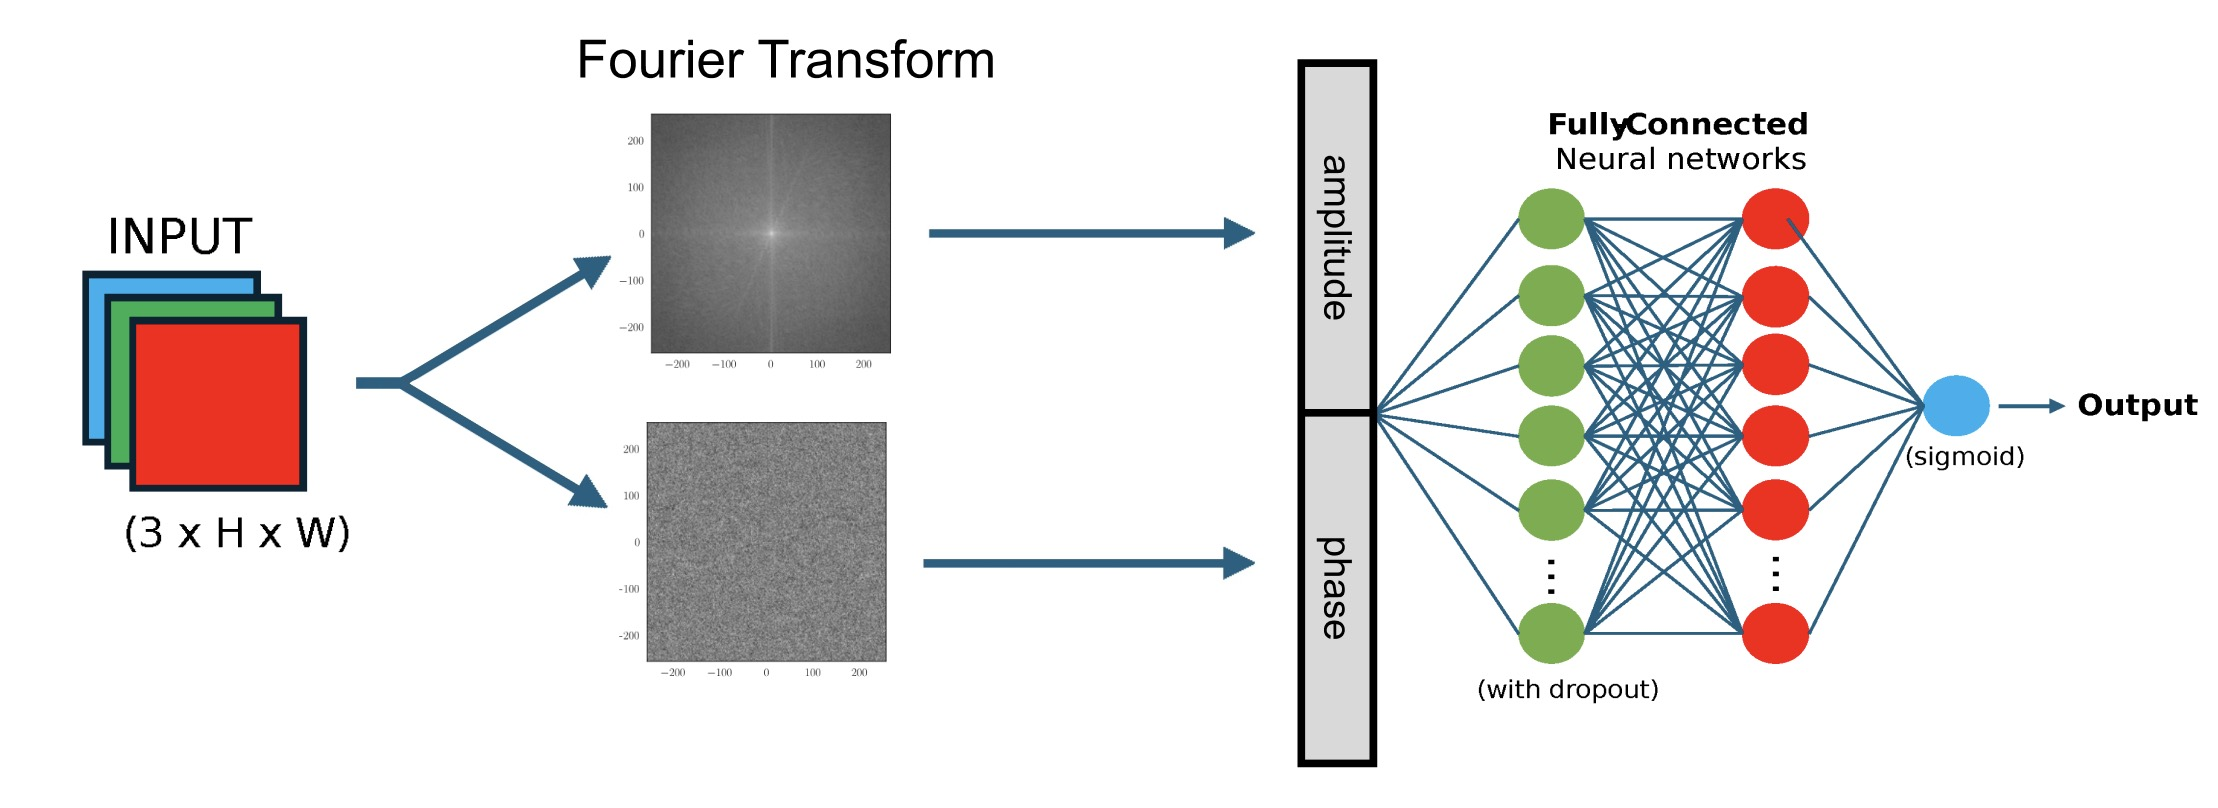
\includegraphics[width=\textwidth]{/Users/sami/Desktop/Brown/Classes/Fall 2024/CSCI 1430/CS1430_Projects/final-project-1430-CV/writeup/Images/Fourier only.jpg}
        \caption{Fourier Transform only model architecture}\label{fig:fig2}

        \includegraphics[width=\textwidth]{/Users/sami/Desktop/Brown/Classes/Fall 2024/CSCI 1430/CS1430_Projects/final-project-1430-CV/writeup/Images/Append figure.jpg}
        \caption{Original CNN with concatenated frequency data model architecture}\label{fig:fig3}

        \includegraphics[width=\textwidth]{/Users/sami/Desktop/Brown/Classes/Fall 2024/CSCI 1430/CS1430_Projects/final-project-1430-CV/writeup/Images/Combined figure.jpg}
        \caption{Combined parallel architectures (Original CNN and fully connected Fourier Transform) model architecture}\label{fig:fig4}
        
        
        \label{fig:vertical_boxed_images}
    \end{minipage}%
\end{figure}

We leveraged the CIFAKE dataset which contained 120,000 total images - 60,000 images are AI-generated and the other half are real \cite{1}. We decided to use this dataset because it was free, publicly available, and easy to access via Kaggle. Furthermore, it seems to be used by many researchers in several research papers we read, supporting its credibility in the field. We used 100,000 images to train the CNN and the remaining 20,000 images were used for testing. Due to our laptops’ hardware limitations, we leveraged Brown’s remote supercomputer, OSCAR, to train our model, especially given the sheer amount of data we were feeding it.

Since we were working on CNN architectures and keeping track of a lightweight image dataset, we decided to repurpose the Homework 5 code for this project, allowing us to work in a familiar environment and focus on training rather than setup.

To test our hypothesis, Fourier Transforms contain frequency information about AI-generated images which could be leveraged to improve classification tasks, we started by reimplementing the architecture outlined in the paper with the highest CIFAKE accuracy, as depicted above (Figure \ref{fig:fig1}). The paper had details about the convolutional blocks and the type of layers used, but their details on the fully connected head were lacking. As a result, we had to perform many tests to identify the best hyperparameters such as learning rate (1e-3), number of epochs (50), and the dropout rate (0.3).

This paper served as a starting point and baseline for our testing, so we decided not to change the hyperparameter values after our initial conclusions. We also did not perform any data augmentation (such as rotation, scaling, etc.) and we preserved the paper’s lightweight architecture style by keeping all subsequent models under 10 million parameters. Furthermore, we didn’t apply any pre-processing techniques to the original image dataset, since the model architecture already seemed to handle the raw data effectively.

We then made our first major architecture modification which aimed to establish whether the Fourier Transform of input images, i.e. their representation in the frequency domain, contained any information that could help differentiate between real and AI-generated images. To test this, we used a simple neural network that took an image, performed a Fourier Transform to extract its amplitude and phase, and ran it through many dense layers to output a prediction.

After obtaining positive results from this exploration, we conducted our first experiment to evaluate the effect of adding this frequency information to the original CNN architecture we recreated from the paper. As seen in Figure \ref{fig:fig3}, we determine the amplitude and phase of the input image, and concatenate it to the flattened output of the convolutional layer. This new vector is then passed through a dense neural network, as was the case in the original paper architecture. We performed an additional baseline test where random noise, instead of the Fourier Transform information, was concatenated with the output of the convolutional layer. This experiment was intentionally designed to add the Fourier information aggressively into the original CNN architecture, as we wanted the dense layer to process both spatial and frequency information at the same time.

Following this experiment, we had a solid idea of the predictive power of the frequency domain of an image. However, we were unsure whether this information was complementary to the spatial information, or if it was a more noisy representation of the data with no added value. To investigate this, we introduced our second experiment, which can be thought of as a combination of the first experiment and the original architecture. As can be seen in Figure \ref{fig:fig4}, we ran the Fourier Transform neural network and the CNN architecture in parallel, and then combined the outputs of both neural networks (respectively size 256 and 128) into a final fully connected neural network. Conceptually, this would enable the “combined” neural network to determine the value of both outputs and decide which one to use, without having to process both the spatial and frequency data at the same time (which was the case in the first experiment). We also conducted a baseline of this experiment using random noise instead of the Fourier, and this enabled us to deduce whether this “combining” network completely excluded the Fourier output, or if it used it to make better predictions.

These experiments were carefully designed to test our architecture, and we detail our findings in the subsequent section.


\section{Results}

\begin{table}[h]
    \centering
    \begin{tabular}{|l|c|}
    \hline
    \textbf{Model} & \textbf{Test Accuracy} \\
    \hline
    \textbf{Original CNN model} (Figure \ref{fig:fig1}) & 98.58\% \\
    \hline
    \textbf{Fourier Transform only} (Figure \ref{fig:fig2}) & 82.53\% \\
    \hline
    \multicolumn{2}{|l|}{\textbf{Concatenated Fourier} (Figure \ref{fig:fig3}):} \\
    \hline
    ~~~~Baseline (Random Noise) & 50.35\% \\
    ~~~~Fourier Transform & 95.36\% \\
    \hline
    \multicolumn{2}{|l|}{\textbf{Combined Parallel Architectures} (Figure \ref{fig:fig4}):} \\
    \hline
    ~~~~Baseline & 98.50\% \\
    ~~~~Experimental conditions & 98.50\% \\
    \hline
    \end{tabular}
    \caption{Model Performance Comparison}
    \label{tab:model-comparison}
\end{table}

The results of the experiments outlined in the previous sections are summarized above (Table \ref{tab:model-comparison}); the following is a more detailed explanation and interpretation of these accuracies.

Our reimplementation of the CNN model (c.f. Figure \ref{fig:fig1}) yielded a test accuracy of 98.58\%. This performance provided a baseline for comparison with the results of our experiments that incorporated Fourier Transform information.

The second baseline we established was with a model architecture using only the Fourier Transform information (c.f. Figure \ref{fig:fig2}) which resulted in a test accuracy of 82.53\%. This moderate accuracy tells us that Fourier Transform information independently holds value in classifying between real and AI-generated images as it was significantly above a random or 50\% accuracy. However, independently, it is less accurate than using convolutional layers on the original images which had an accuracy of 98.58\%. This was expected given the superiority of CNN architectures when dealing with image data.

As discussed in the aforementioned “Method” section, our first experiment combined the Fourier Transform information with the output from the convolutional layers (c.f. Figure \ref{fig:fig3}). Our baseline conditions, which appended random noise to the convolutional output vector, performed with a near random classification accuracy of 50.35\%. However, our experimental conditions, which appended the Fourier Transform vector, resulted in an accuracy of 95.36\%. While the addition of both types of information, noise and Fourier Transform, reduced the accuracy of the model from the original CNN model, the noise essentially rendered the model useless while the Fourier Transform information only reduced accuracy slightly. These results suggest that the Fourier Transform information, although not able to improve the accuracy, did contain predictive information.

These results suggest that frequency information has predictive potential for AI-generated image detection, but we wanted to determine whether it provided added value to the CNN architecture. Our second experiment combined both Fourier and CNN architectures into one model (c.f. Figure \ref{fig:fig4}). The results of both frequency information and random noise yielded the same accuracy as the very first reimplemented CNN architecture - 98.5\%. This lack of a difference in accuracy between the baseline and experimental group is different from the significant difference observed in the concatenation experiment (c.f. Figure \ref{fig:fig3}). This suggests that when the information is directly appended into the same fully connected layers as the convolutional layer, the model uses all of the information provided, causing there to be a large accuracy distinction in experiment 1 between the baseline and experimental group. However in experiment 2 when the model was given these outputs separately it was able to choose the information to use to predict classification. Given the same accuracies for the baseline and the experimental group were both 98.50\%, it’s clear the model ignored the noise and Fourier Transform information and only used the convolutional layer information regardless.


%-------------------------------------------------------------------------
\subsection{Technical Discussion}

The focus of our work for this project was around designing simple and insightful experiments. To do so, we performed many tests to determine architectural features, while also keeping the number of parameters low, all of which resulted in many small variations between experiments.

A notable example of this is our varying fully connected neural network sizes. The initial CNN head was what we considered normal, with perceptron numbers going from 256 to 1 with steps of ½. The Fourier-only fully connected network saw an additional 512 dense layers being added to ensure meaningful patterns were extracted from the magnitude and phase features of input images.

The most interesting experiments we undertook were for our “combining” architecture (c.f. Figure \ref{fig:fig4}). A big challenge we had was determining the size of the parallel dense layer outputs. Given that we wanted to append them together, and pass them through a third fully connected network, their respective size, and respective proportions were very important. What we initially noticed was that a single prediction output from both architectures (i.e. each outputting a prediction of the image realness, both then concatenated and passed through the “combining” network), resulted in very poor accuracy. Given that this “decision forest” style architecture provided poor results, so we turned to larger output sizes to allow the combining network to extract more information from each architecture. This provided better results, and after experimenting with many splits, the 1:2 ratio between Fourier output and CNN output seemed to work best. However, given that this architectural design was empirically determined, and was inspired by conceptual intuition, we are unsure if a “combining” neural network was the best option, or if other types of layers or blocks would’ve been more effective (e.g. introducing an attention layer).

Another interesting aspect of the original CNN architecture, and our subsequent experiments, was that, although we had strong performances, often exceeding 95%, we didn’t succumb to overfitting. The gap between training and validation accuracy was very small, as can be seen in Figure \ref{fig:fig5} for the original CNN accuracy.

Using the CIFAKE dataset, we also faced constraints in hyperparameter optimization due to limited GPU resources, despite leveraging Brown’s OSCAR supercomputers. It was not feasible to hyperparameter optimize every aspect of the model; not only did we have to adjust hyperparameters for the Fourier-enhanced model, but we also had to apply these changes to the baseline model. This limitation forced us to make decisions about which hyperparameters and model parameters to tune, focusing on the most impactful ones, such as dropout rate and epoch number.


%------------------------------------------------------------------------
\section{Conclusion}

In this paper, we created and evaluated an AI-Generated Image Detector designed to distinguish real images from AI-generated ones. Our experiments demonstrated that incorporating Fourier features into the detection pipeline provided valuable insights, although the overall accuracy depended mostly on the CNN architecture. While our baseline model already achieved high accuracy, the addition of Fourier Transform features revealed weaknesses in specific scenarios, even though they are able to detect small differences in patterns and frequencies found in synthetic images.

A limitation of our project is the use of the CIFAKE dataset, which contains only 32×32 resolution images. Another limitation is that while this dataset is relatively new, it does not account for the significant advances in generative AI made in the last year. Hence, while this dataset allowed for efficient training and testing, it does not represent the variety or complexity of real-world images, limiting the generalizability of our findings. Future research should prioritize datasets with higher resolutions and more diverse content to ensure better performance in real world images/applications. As generative AI continues to evolve, solutions like the one proposed in this paper will play an important role in preserving digital authenticity and societal trust.




{\small
\bibliographystyle{plain}
\bibliography{ProjectFinal_ProjectReportTemplate}
}

\vspace{0.2cm}
\section*{Appendix}

\vspace{0.3cm}

\subsection*{Team contributions}

\vspace{0.1cm}

\begin{description}

\item[Everest Yang:] I developed the code for integrating the Fourier Transform into our model, including the implementation for concatenating the flattened vector dimensions. Additionally, I conducted an extensive review of related works and research papers to identify optimal CNN architectures. I also contributed significantly to the writing of the paper, specifically on the Introduction, Related Works, Technical Discussion, Conclusion, and key parts of the Method section. Furthermore, I formatted the entire document into a comprehensible research paper format using LaTeX and a .bib file for our references.

\item[Tanay Subramanian:] I was responsible for finding literature concerning current research concerning neural networks and the integration of Fourier transforms into classification tasks. Additionally, I helped develop the code for the baseline model architecture, in addition to working on the final paper, contributing to the Abstract, Introduction, Methods, and Conclusion sections. I also worked extensively on the final presentation slides, helping summarize our research in a concise and visually appealing manner.

\item[Sujith Pakala:] Once we realized that our project would require more computing power than our computers or Google Colab would allow, I took on the role of understanding and debugging our set-up with Oscar to be able to test our models in a time efficient manner. I also spearheaded the development of the code for our baseline without the fourier transform and the code for just using the fourier transformation after investigating architectures used historically in the literature. I also worked with Sami to design our “experiments” and created the graphs used in the report. 

\item[Sami Nourji:] I took on the role of Project Manager for this final project, helping develop the project idea, and managing the allocation of tasks among teammates. My work within the project involved developing the Fourier experiments, model architectures, and training the model. I also worked on interpreting the model results and formulating the write up conclusion



\end{description}

\end{document}
